\chapter{Making a Figure with Width Based on Page Size}
\label{apdx:appendixa}

\section{Width Based on Page Size Figure Example} \label{sec:appendixa_figure_example}
Here's an example of a figure whose width depends on the width
of the page. You can see it as Figure~\ref{fig:appendix_some_pic}. This also shows another citation \cite{aeyels86local}.

\begin{figure}[htbp]
  \centering
  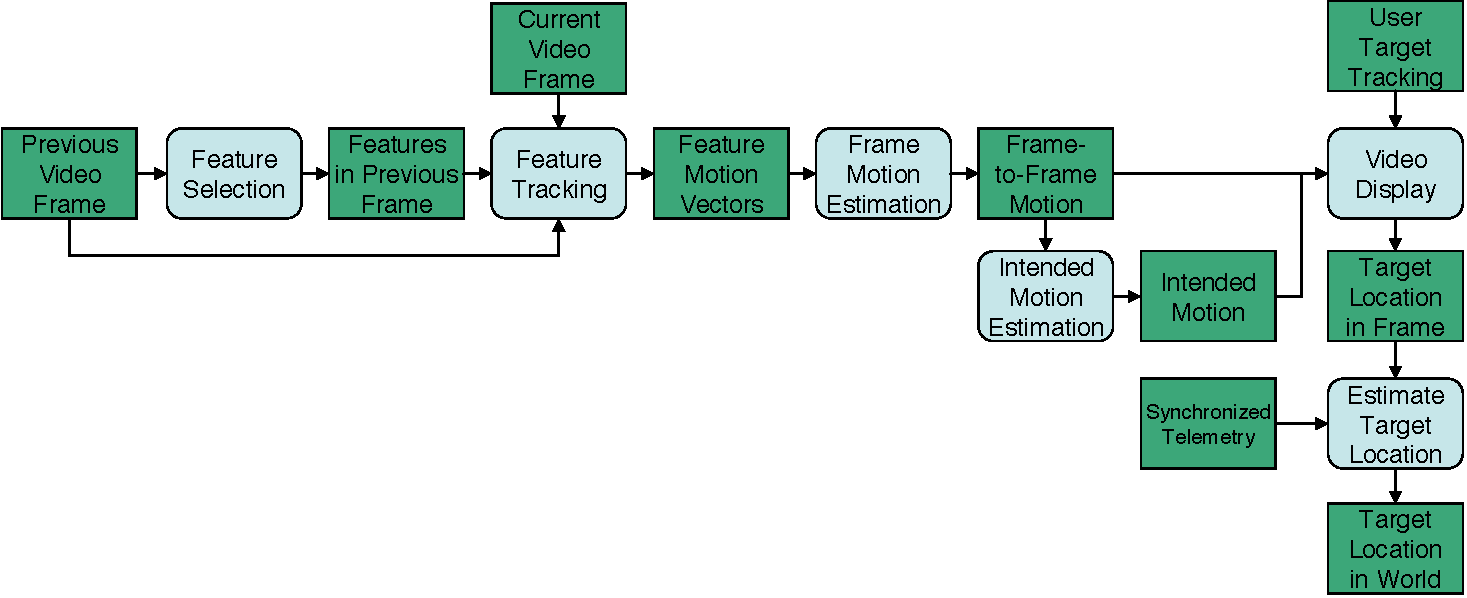
\includegraphics[width=0.45\textwidth]{images/some_pic}
  \caption[Example figure whose width depends on page size]{
    This is an example of a figure whose width will be 45\% of the
    width of the page. If you'd like to see a figure with a fixed
    width then you can see it as Figure~\ref{fig:intro_stuff} in
    Section~\ref{sec:intro_figure_example} of Chapter~\ref{chp:chapter1}.}
  \label{fig:appendix_some_pic}
\end{figure}